\documentclass[prb,twocolumn]{revtex4-2}
\usepackage{graphicx}
\usepackage{amsmath}
\usepackage{amssymb}
\usepackage{float}
\usepackage{epstopdf}

\begin{document}
\title{Assignment 6 Extra Credit}

\author{James Lawton}
\affiliation {
Physics Department, Virginia Tech, Blacksburg, Virginia 24061, USA\\
}


\begin{abstract}
Abstract: Using a Genetic Algorithm to find the Platonic solids
\end{abstract}

\maketitle

\section{Genetic Algorithm}

\noindent

Here a genetic algorithm is used to find the Platonic solids

There are four basic steps to a genetic algorithm:

\begin{enumerate}
    \item Creating a gene pool
    \item Encoding a configuration
    \item Selection operation
    \item Crossover operation
    \item Mutation operation
\end{enumerate}

I used most of the same code from the Thomson java file with a few key 
differences. For each point I found a list of the points closest to it with 
equal distance and made sure that the more that were equally distant it would
reduce the energy cost. This pushes the algorithm to find shapes with regular 
polygons as faces.

\subsection{Tetrahedron}
\begin{figure}[H]
    \centerline{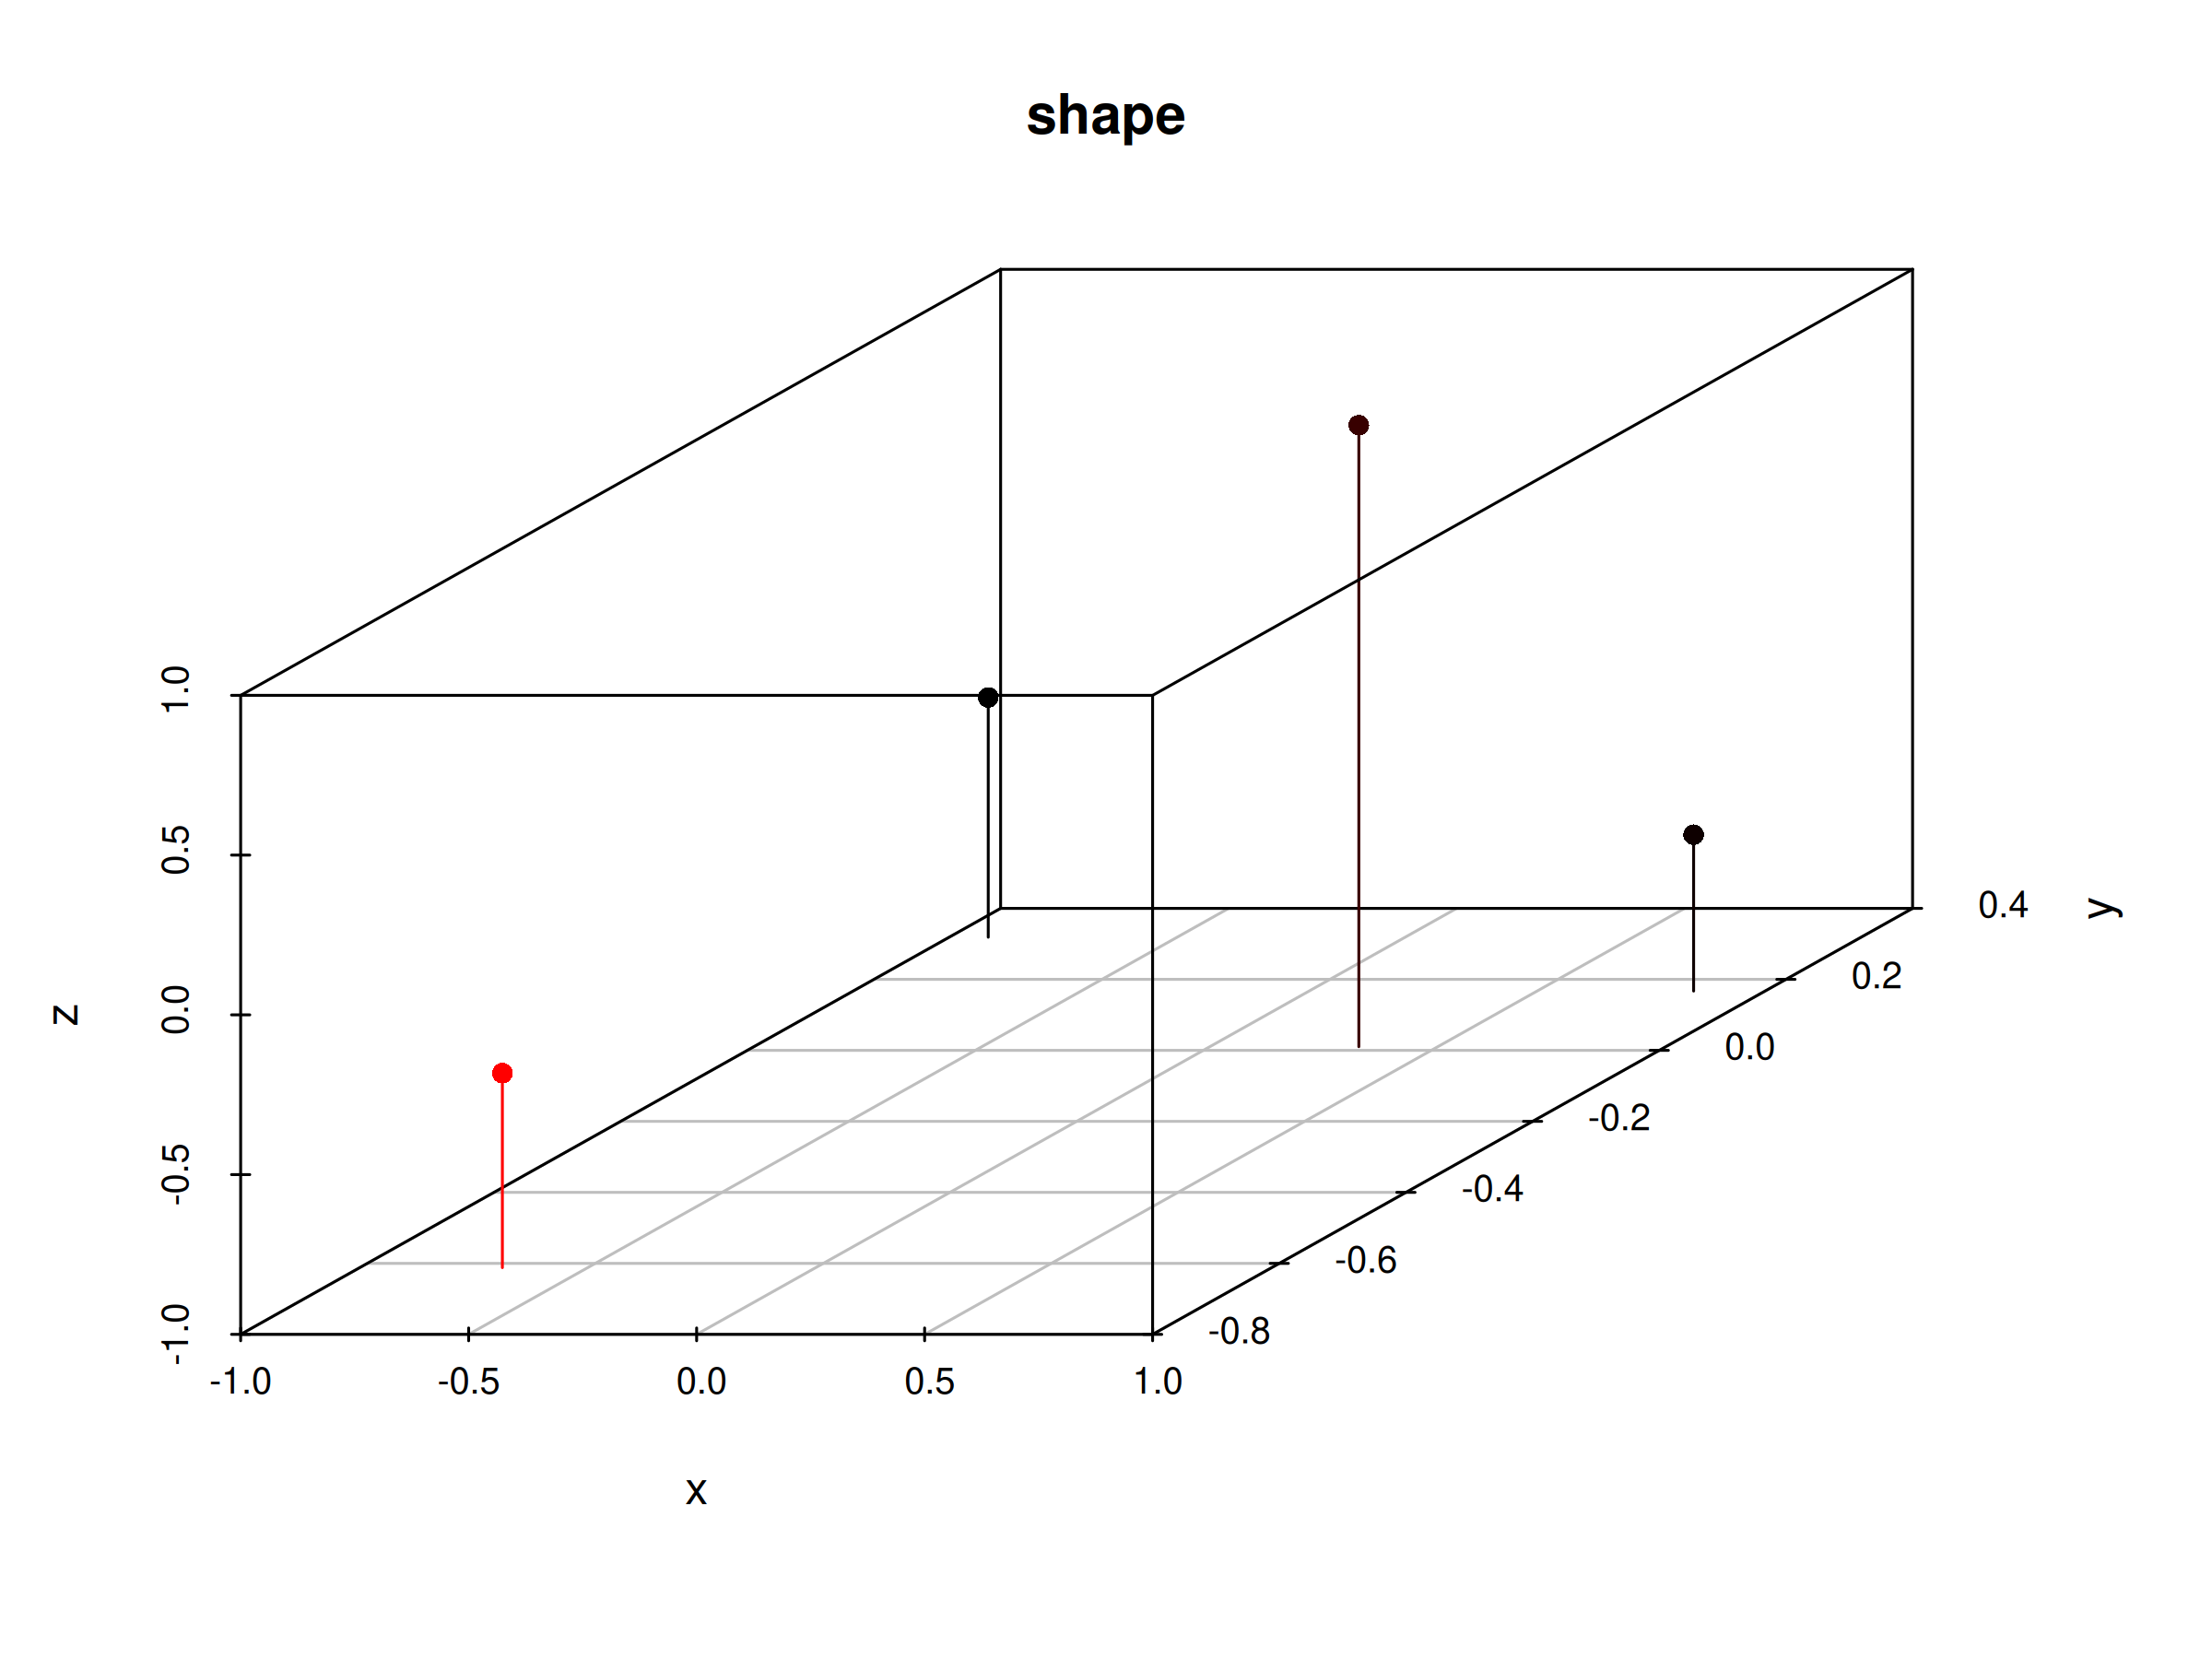
\includegraphics [width=3 in] {img/tetra.png}}
    \caption{Tetrahedron} \label{q1}
\end{figure}

\subsection{Octahedron}
\begin{figure}[H]
    \centerline{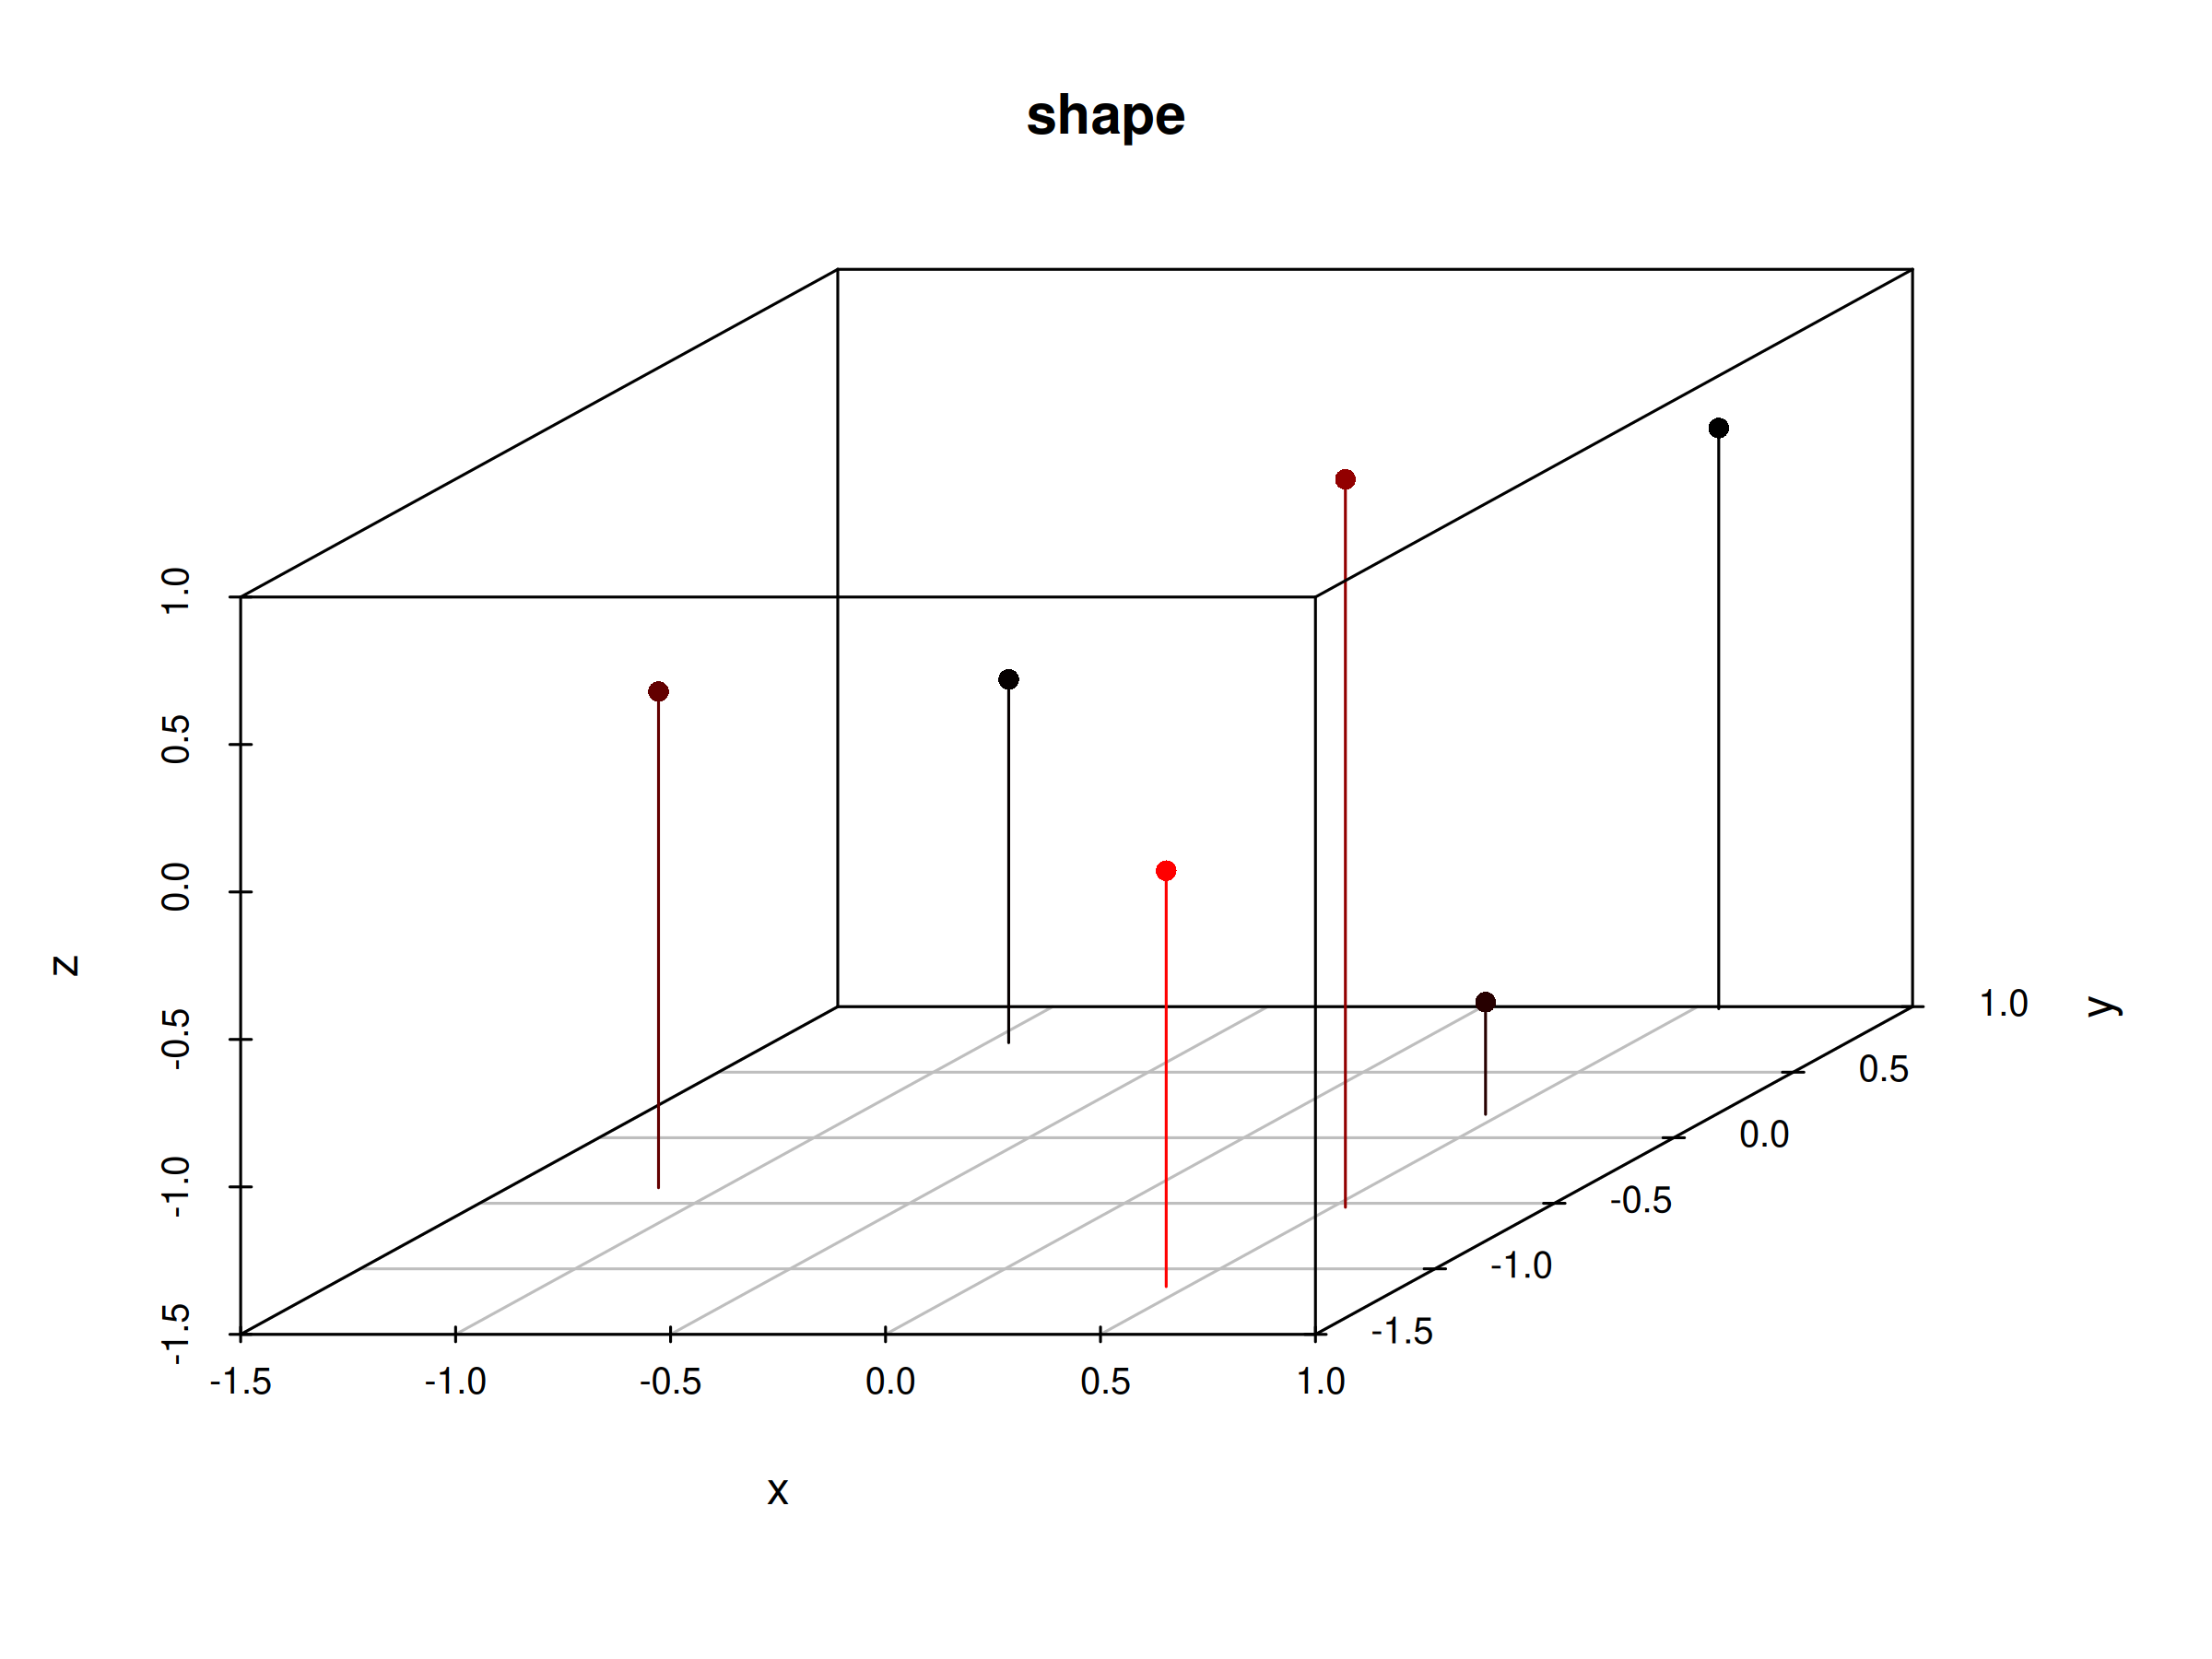
\includegraphics [width=3 in] {img/octa.png}}
    \caption{Octahedron} \label{q1}
\end{figure}

\subsection{Cube}
\begin{figure}[H]
    \centerline{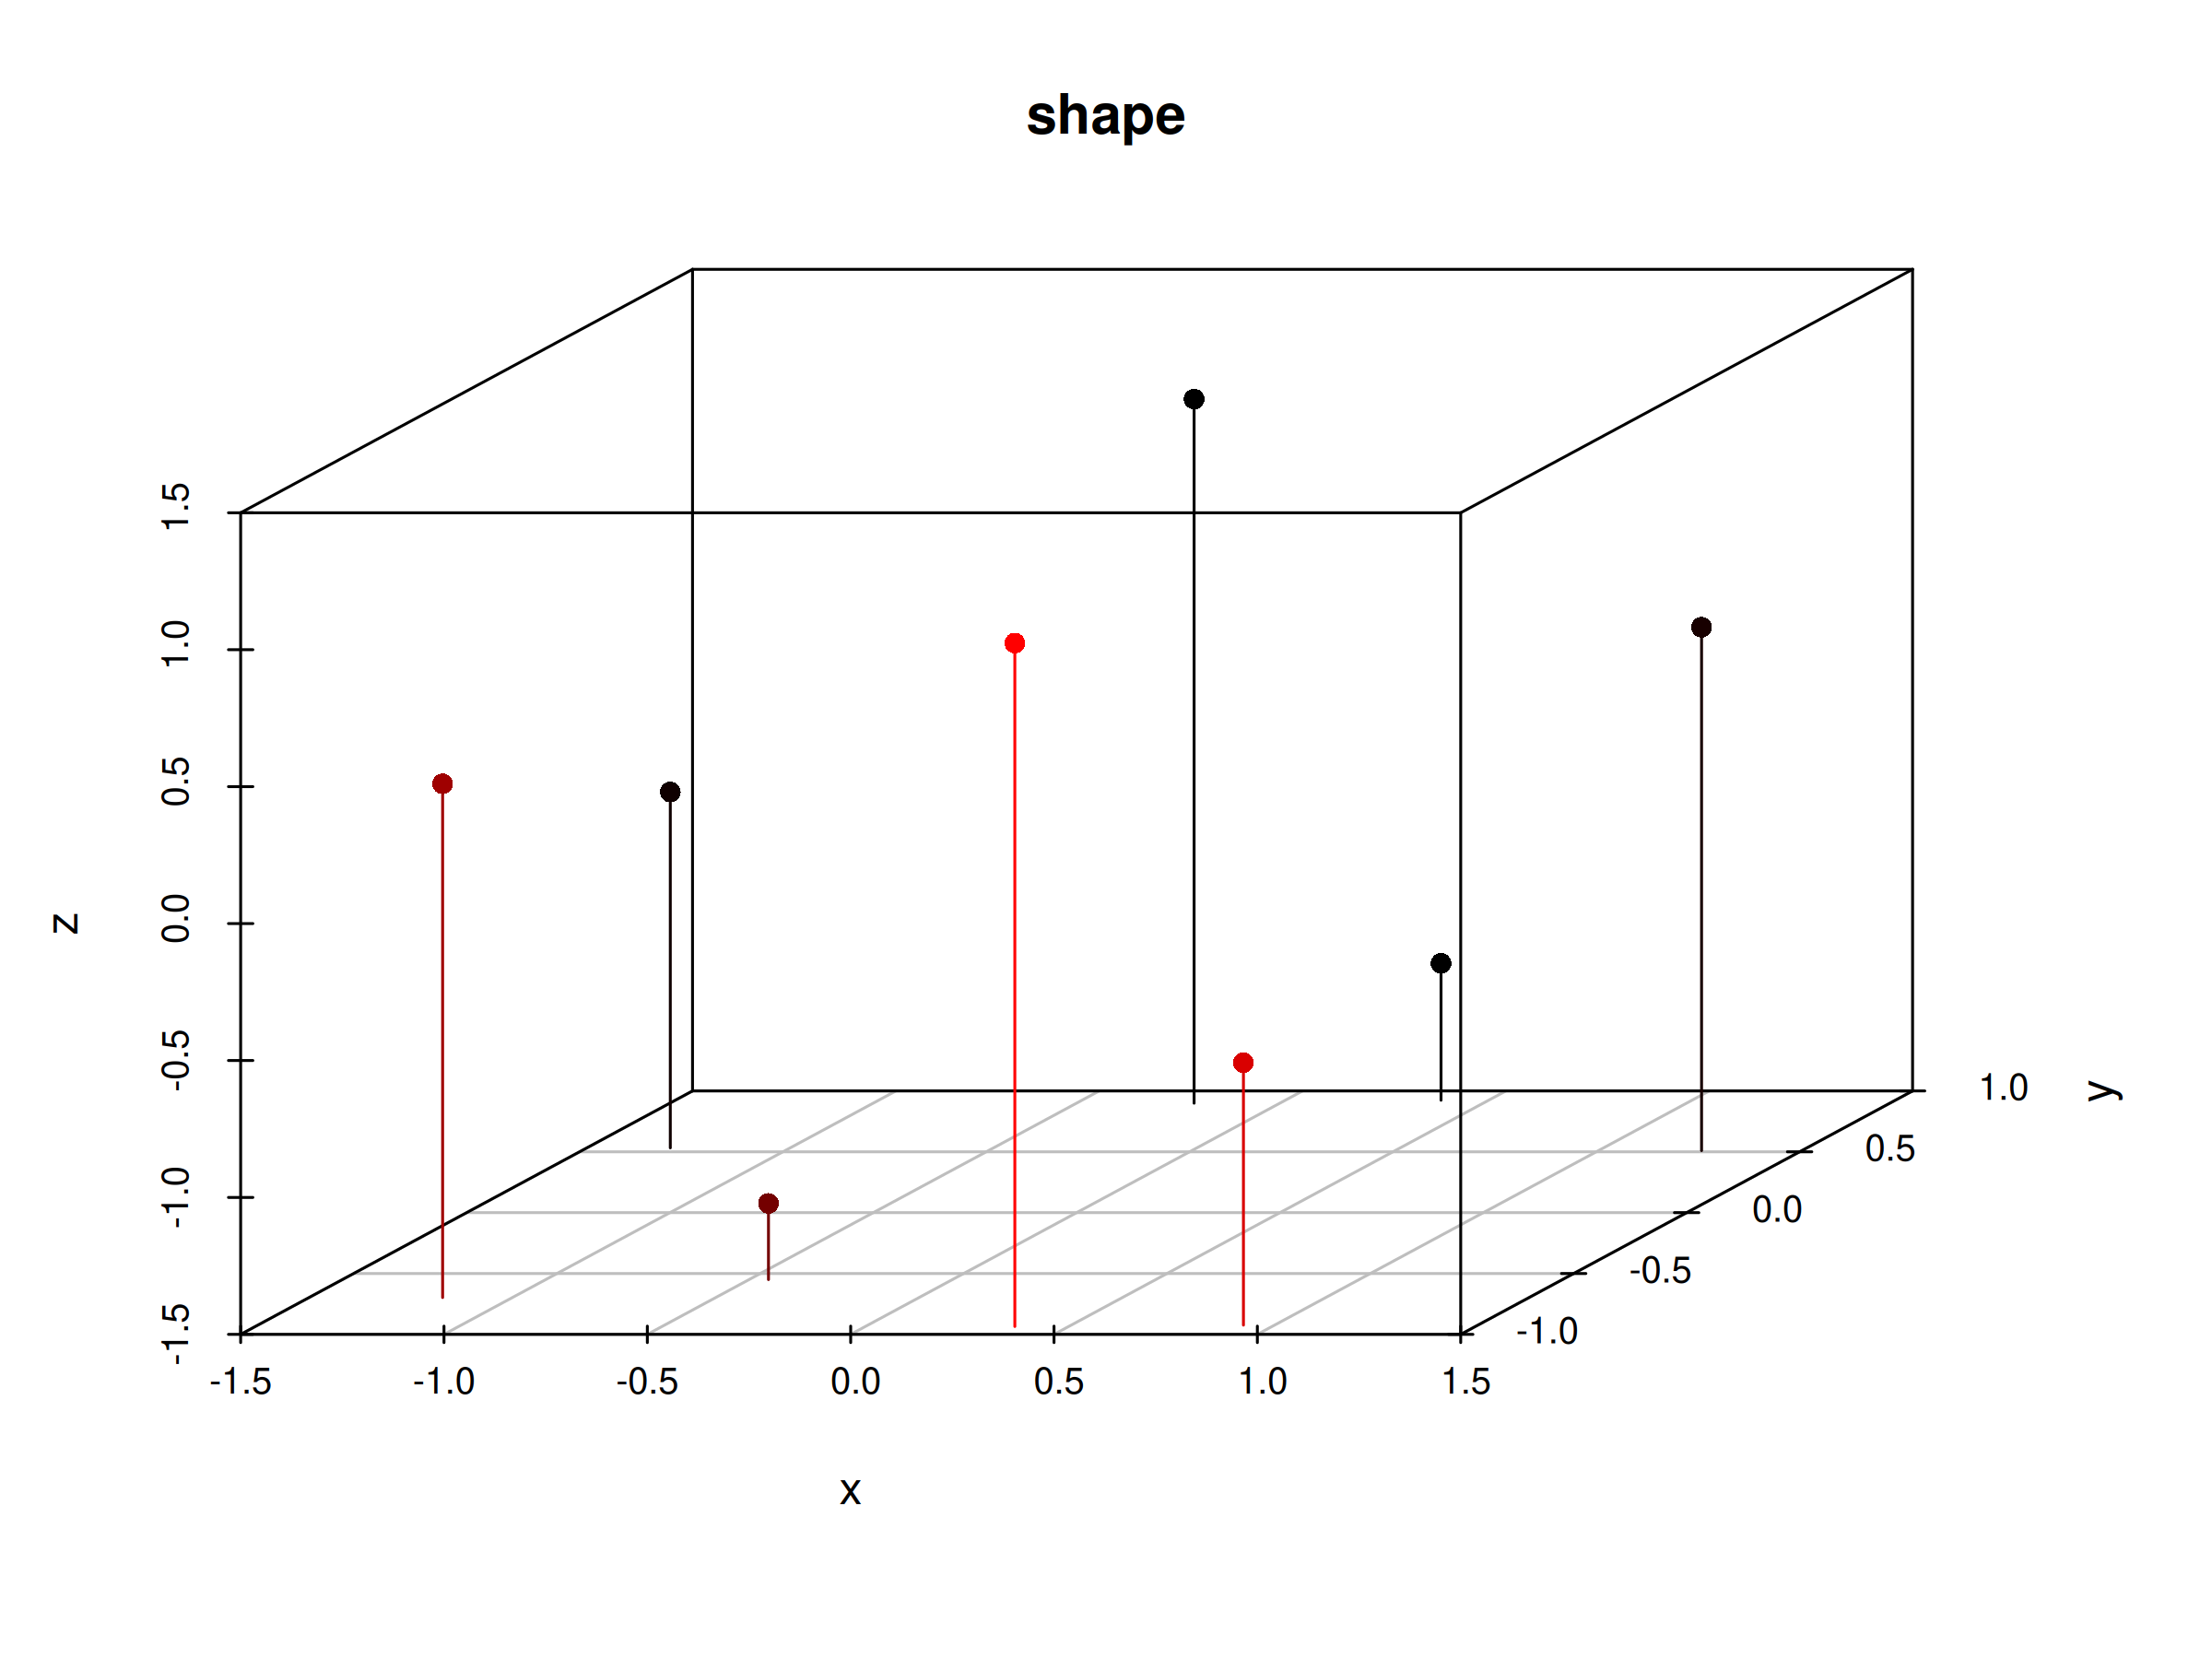
\includegraphics [width=3 in] {img/cube.png}}
    \caption{Cube} \label{q1}
\end{figure}

\subsection{Icosahedron}
\begin{figure}[H]
    \centerline{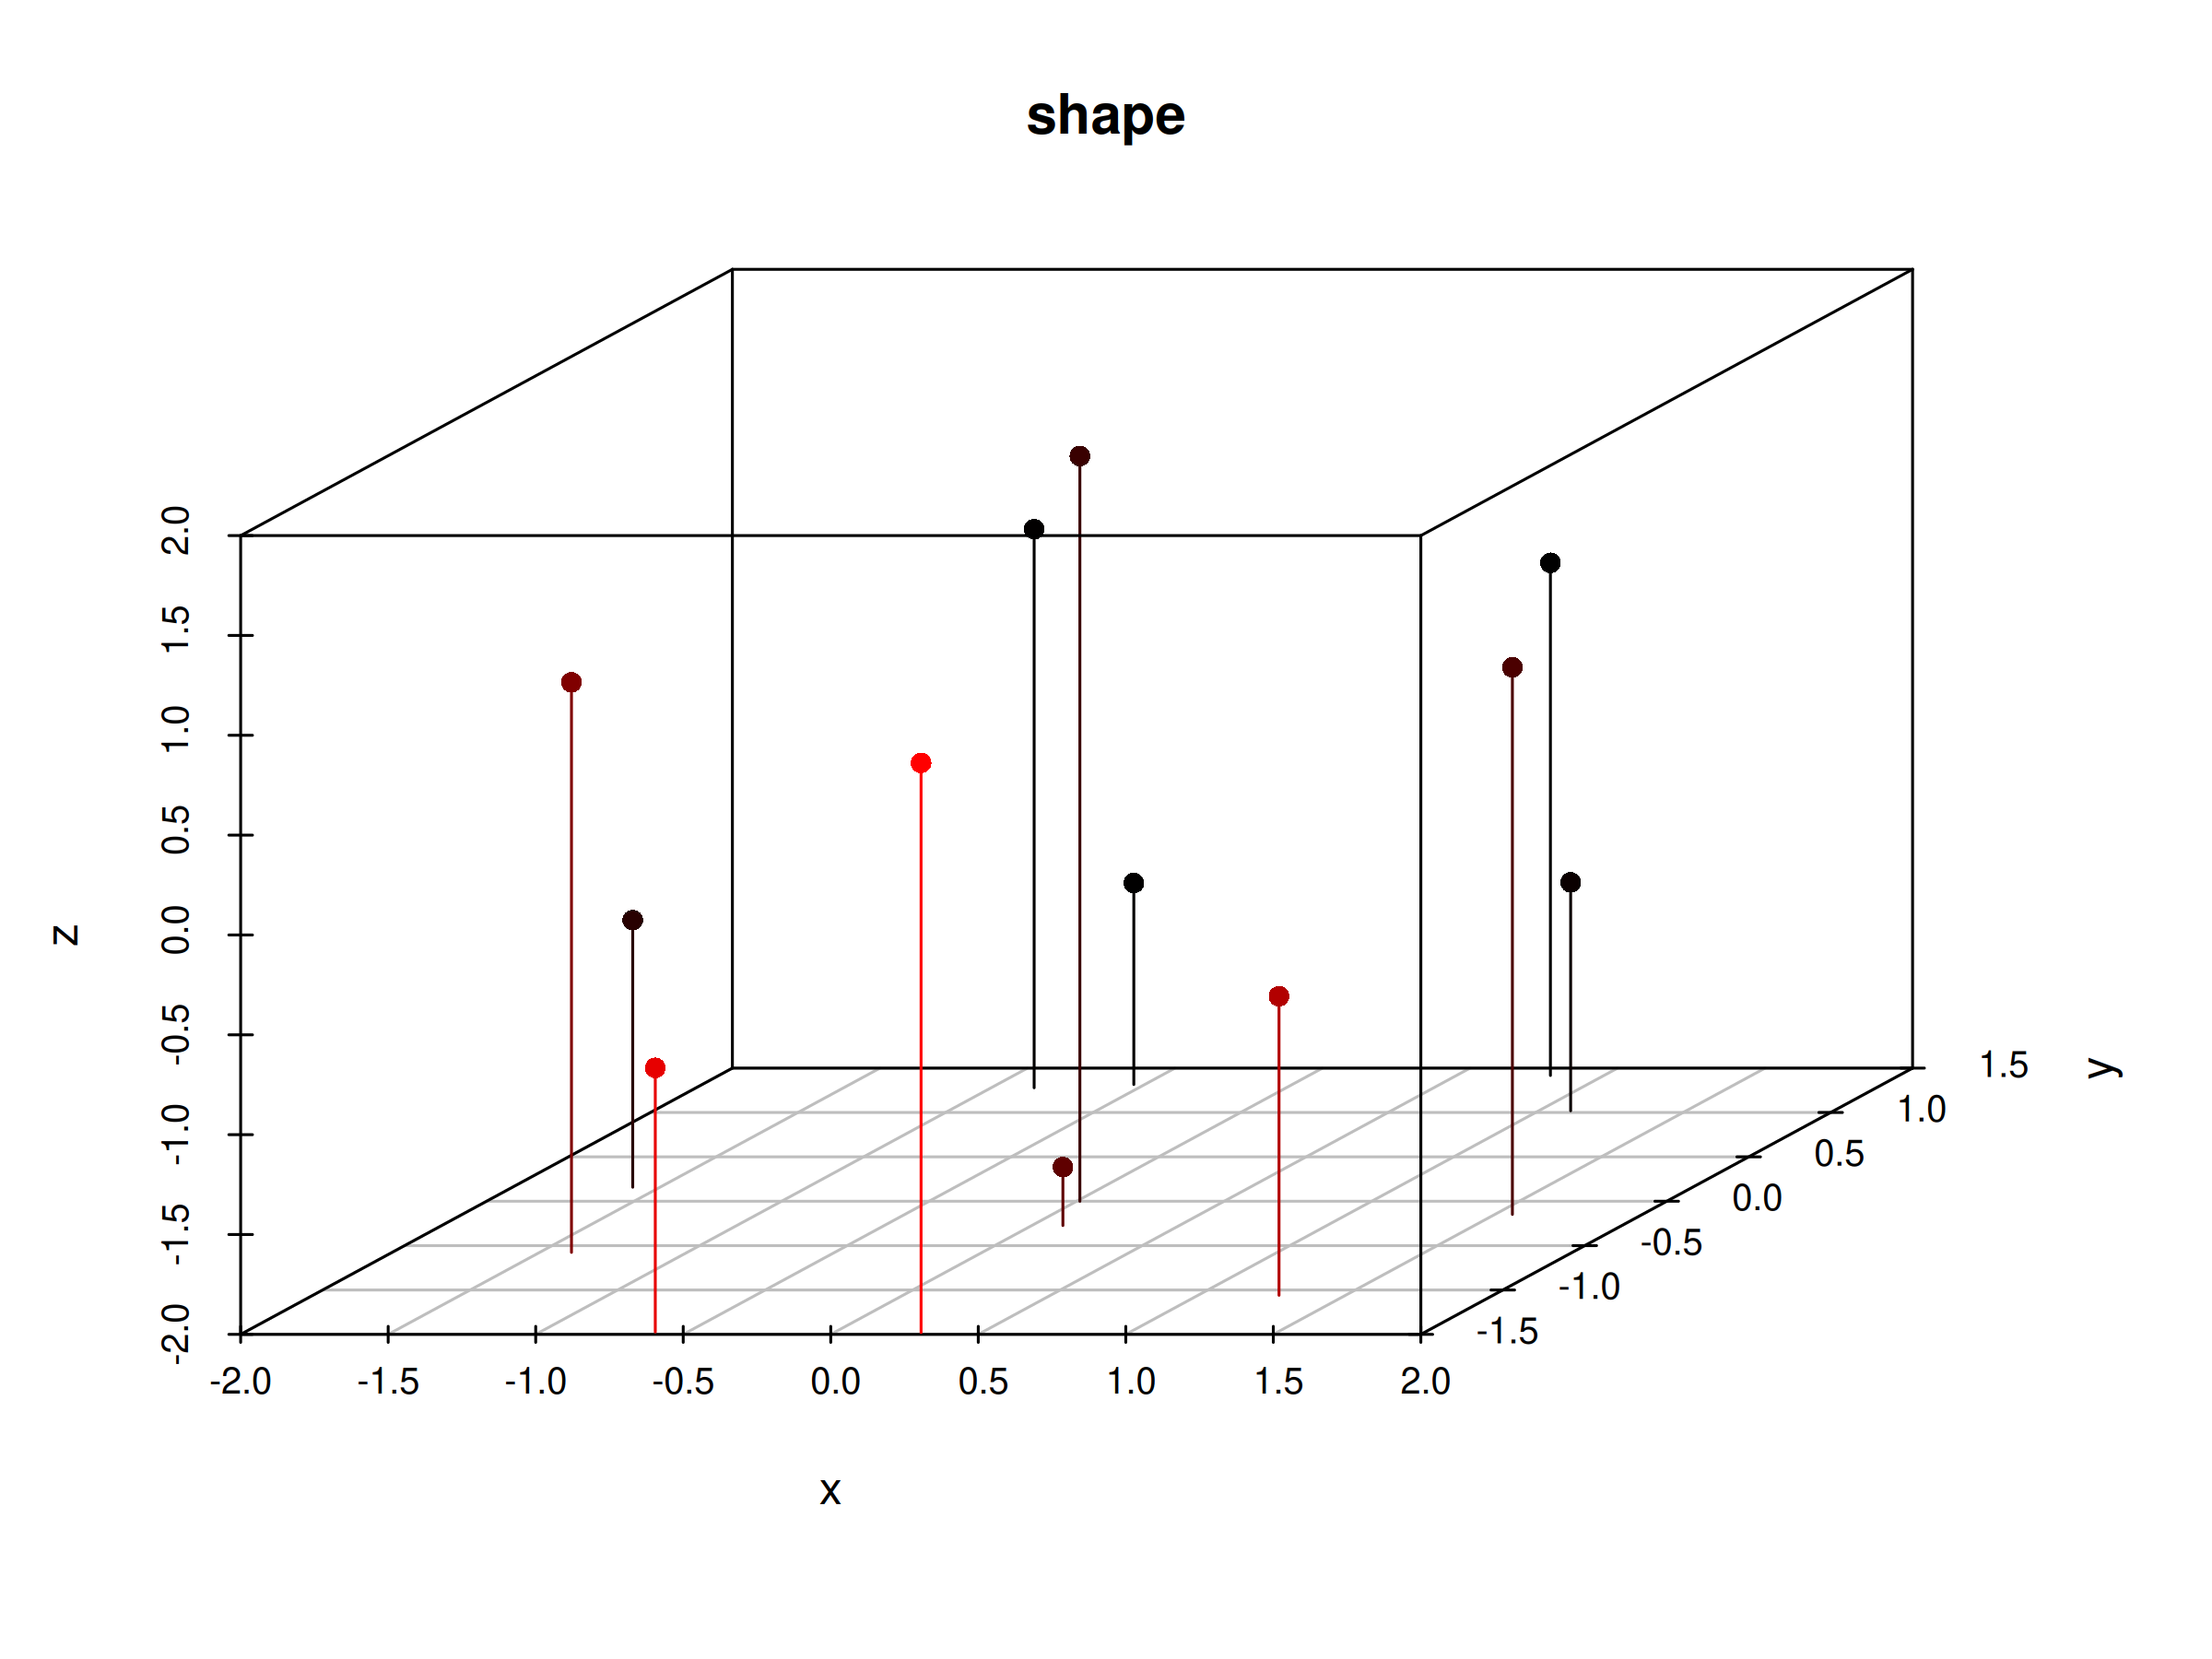
\includegraphics [width=3 in] {img/icosa.png}}
    \caption{Icosahedron} \label{q1}
\end{figure}

\subsection{Dodecahedron}
\begin{figure}[H]
    \centerline{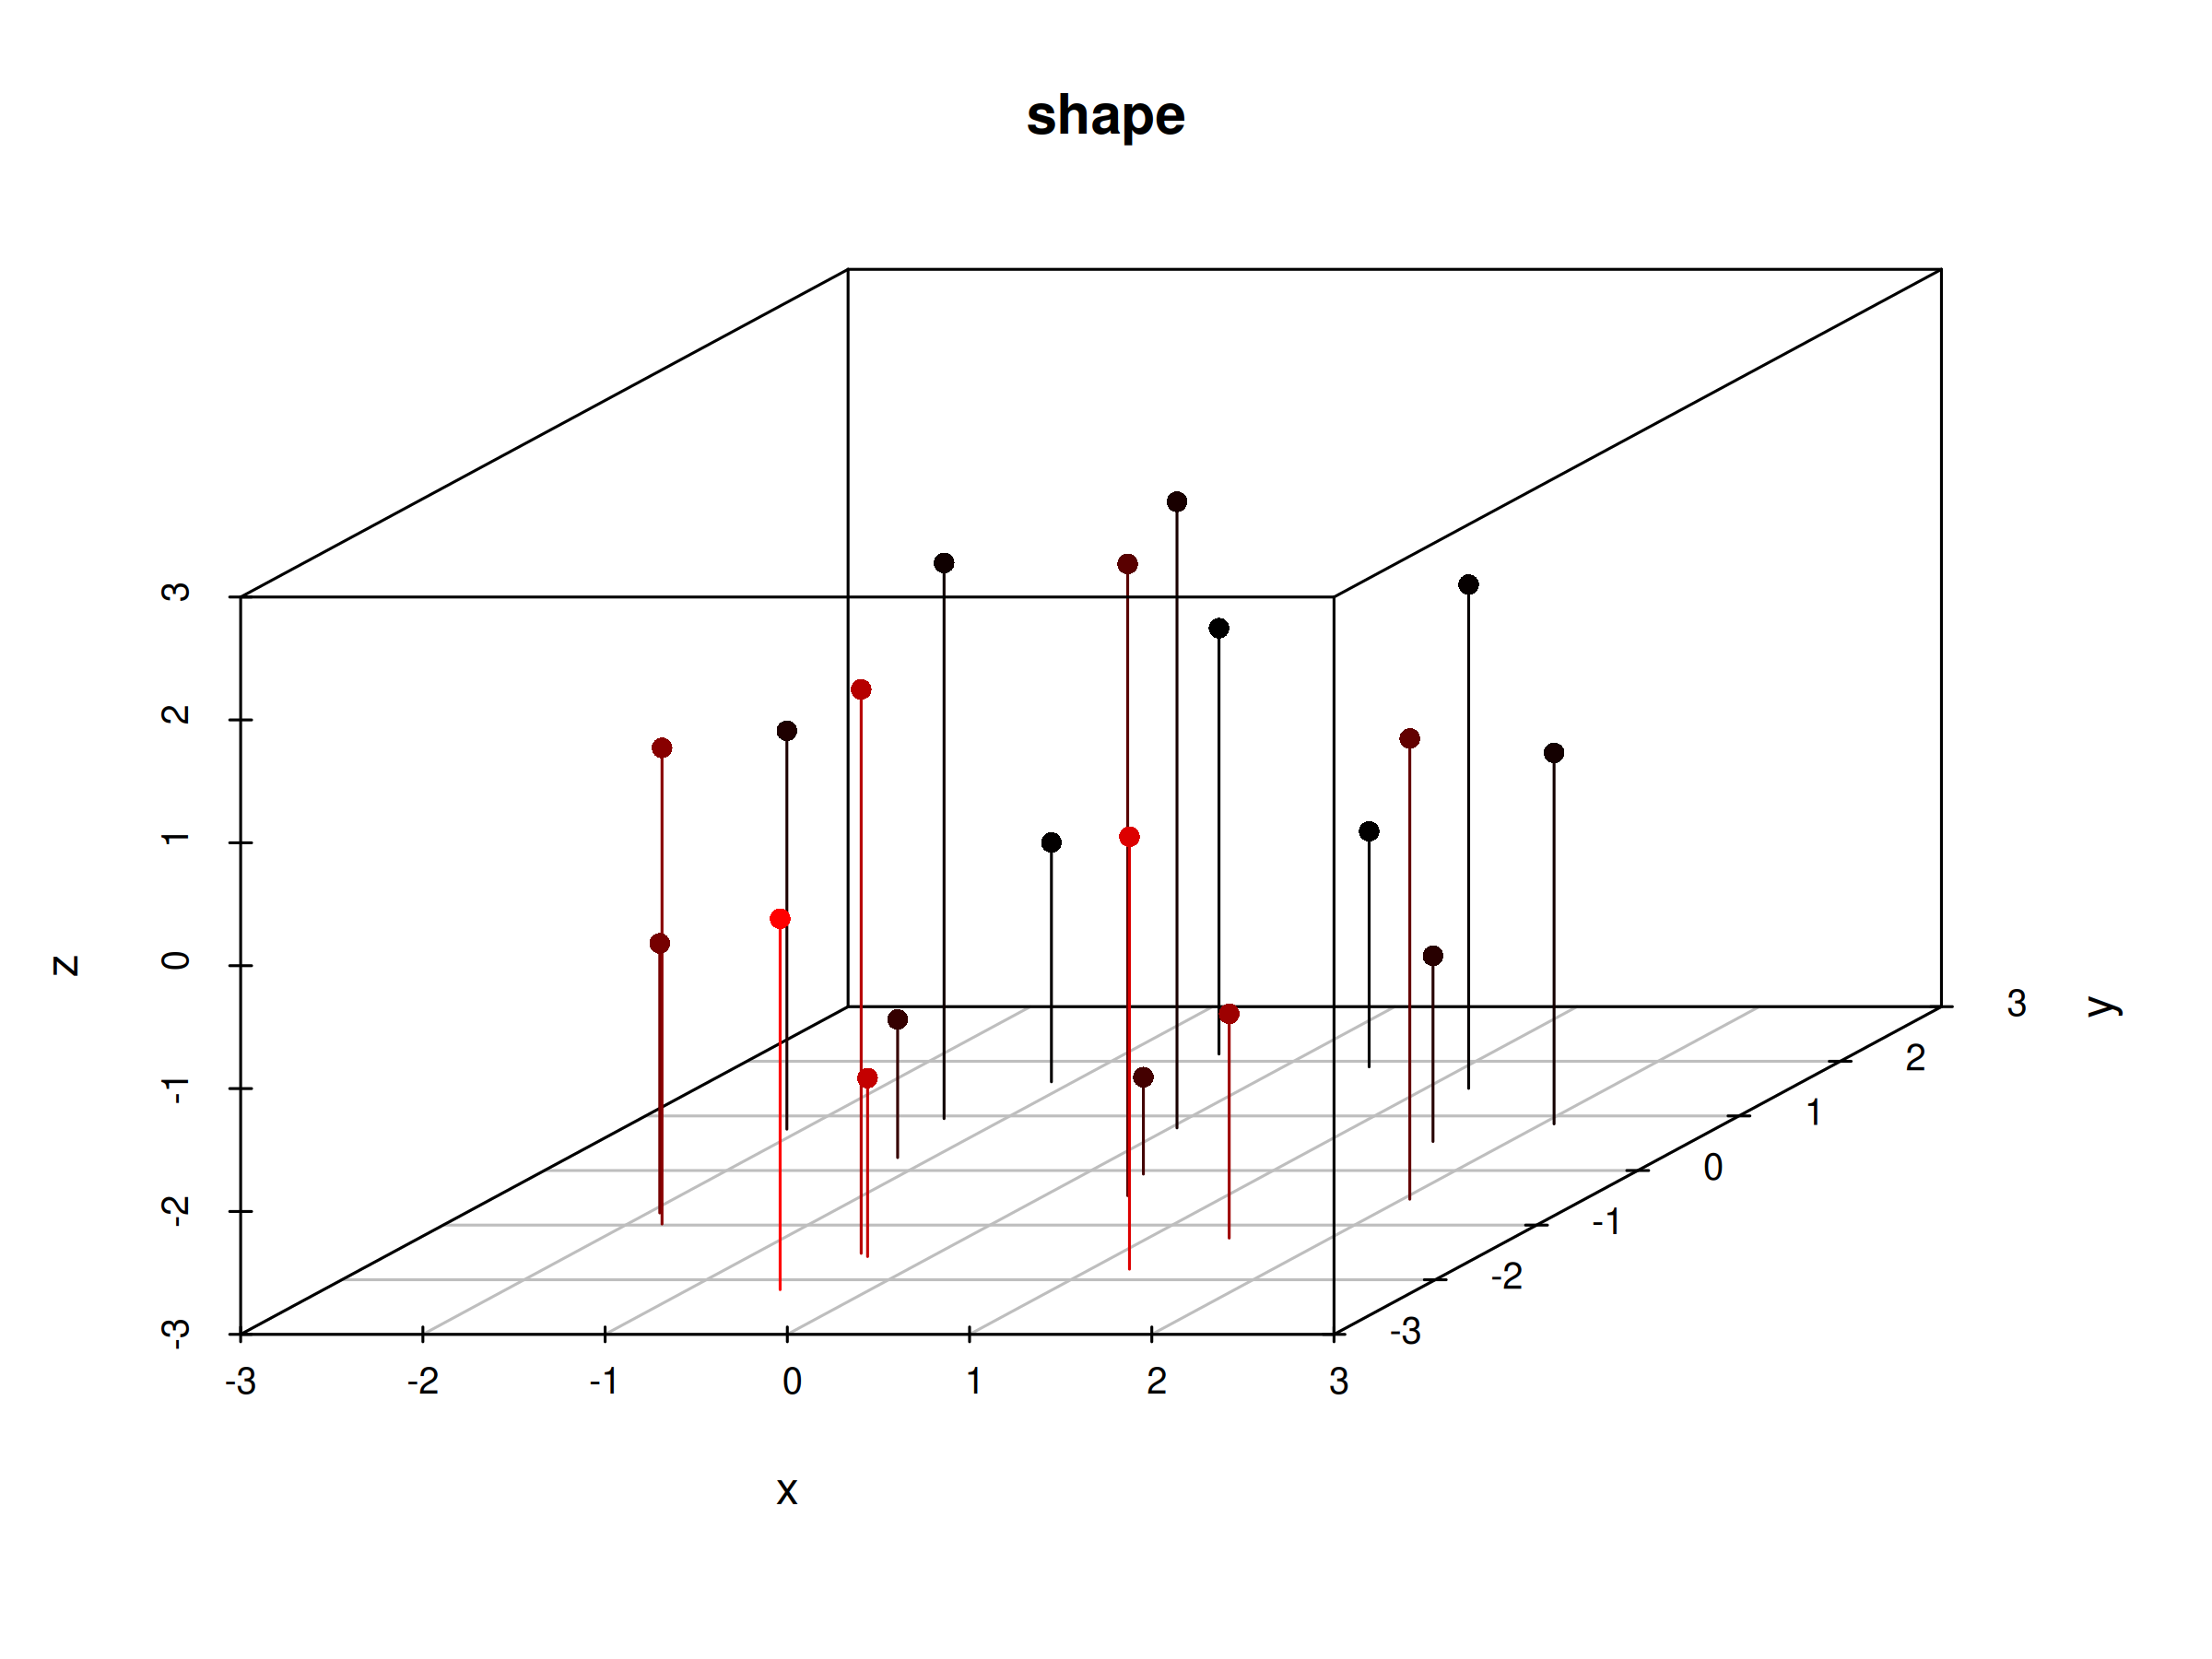
\includegraphics [width=3 in] {img/dodeca.png}}
    \caption{Dodecahedron} \label{q1}
\end{figure}


\begin{thebibliography}{99}

\bibitem{thecoursetext} T. Pang, \emph{Introduction to Computational Physics},
    Cambridge University Press (2006).

\end{thebibliography}

\end{document}
